% -*- Mode:TeX -*-

%% IMPORTANT: The official thesis specifications are available at:
%%            http://libraries.mit.edu/archives/thesis-specs/
%%
%%            Please verify your thesis' formatting and copyright
%%            assignment before submission.  If you notice any
%%            discrepancies between these templates and the 
%%            MIT Libraries' specs, please let us know
%%            by e-mailing thesis@mit.edu

%% The documentclass options along with the pagestyle can be used to generate
%% a technical report, a draft copy, or a regular thesis.  You may need to
%% re-specify the pagestyle after you \include  cover.tex.  For more
%% information, see the first few lines of mitthesis.cls. 

%\documentclass[12pt,vi,twoside]{mitthesis}
%%
%%  If you want your thesis copyright to you instead of MIT, use the
%%  ``vi'' option, as above.
%%
%\documentclass[12pt,twoside,leftblank]{mitthesis}
%%
%% If you want blank pages before new chapters to be labelled ``This
%% Page Intentionally Left Blank'', use the ``leftblank'' option, as
%% above. 

\documentclass[12pt,vi,twoside]{mitthesis}
\usepackage[paper=a4paper,top=6cm,bottom=2.2cm,right=0.83cm,left=3.47cm]{geometry}% http://ctan.org/pkg/geometry
\usepackage{lgrind}
%% These have been added at the request of the MIT Libraries, because
%% some PDF conversions mess up the ligatures.  -LB, 1/22/2014
\usepackage{cmap}
\usepackage[T1]{fontenc}
%% Package "lmodern" added by user request see ServiceNow INC0396734 -OT, 4/29/2020
\usepackage{lmodern}
\pagestyle{plain}
\usepackage{tikz}
\usepackage{pdfoverlay}
\usepackage[ddmmyyyy]{datetime}
\renewcommand{\dateseparator}{.}
\usepackage{float}
\usepackage{amsmath}

\def\abstract{
\vspace{5cm}
\begin{center}%
{\bfseries \abstractname\vspace{-.5em}}%
\end{center}
\quotation
}
\def\endabstract{\par
\endquotation
}


\begin{document}
% \newgeometry{top=6cm,bottom=2.2cm,right=0.83cm,left=3.47cm}
\pagestyle{empty}
% \pdfoverlaySetPDF{cover.pdf}
\begin{center}

% {\large \textbf{PRACA DYPLOMOWA MAGISTERSKA}}
% \vspace{6cm}

{\large \textbf{RAPPORT DE STAGE}}
\vspace{8cm}

{\fontsize{18}{18}\selectfont \textbf{Hybrid neural networks for anomaly detection in~cyber-physical systems}}
\end{center}
\normalsize

% \vspace{6cm}
% \textbf{Wydział Fizyki Technicznej, Informatyki i Matematyki Stosowanej \\
% Promotor:} dr hab. inż. Aneta Poniszewska-Marańda\\
% \textbf{Dyplomant:} inż. Ramzi Hadrich\\
% \textbf{Nr albumu:} 227488\\
% \textbf{Kierunek:} Informatyka\\
% \textbf{Specjalność:} Computer Science \& Information Technology\\
% \begin{center}
%     Łódź, \today r.
% \end{center}

\vspace{8cm}
\noindent Ramzi HADRICH \\
\textbf{Entreprise:} LORIA\\
\textbf{Tuteur Entreprise:} Abdelkader LAHMADI\\
\textbf{Tuteur ENSEM:} Radu RANTA\\
\textbf{Filière:} ISN\\
\begin{center}
    \today
\end{center}

% First copy: start a new page, and save the page number.
\cleardoublepage
\newgeometry{top=2.2cm, bottom=1.5cm, outer=1cm, inner=2.1cm}
% Uncomment the next line if you do NOT want a page number on your
% abstract and acknowledgments pages.
\begin{abstract}
Nowadays cyber-physical systems are widely used in different application domains. In parallel, machine learning algorithms are used widely to detect the anomalies in the behaviour of these systems. However, this detection is limited to two states: normal behaviour and faulty functioning. This work aims to extend this detection to differentiate between attacks and normal faults. In first place, a power system is described as an example to work on. Then, various machine learning algorithms are evaluated on the given datasets, and this using two machine learning toolkits - scikit-learn and Weka. Later, various tools for feature analysis are presented and an algorithm to find the features that contributed the most into the false predictions is described. Finally, three solutions to the initial problem are presented and evaluated - one solution uses the features found in the previous step and modifies their values, the second shrinks the samples from the dataset to have only the previously mentioned features and evaluates the distance between those samples and the third solution uses the Hidden Markov Model. The test have shown that the best performing solution was the second, even if the gain in accuracy is not very significant.  
\end{abstract}

\newpage
\renewcommand{\abstractname}{Résumé}
\begin{abstract}
De nos jours, les systèmes cyber-physiques sont largement utilisés dans différents domaines d'application. Parallèlement, les algorithmes d'apprentissage automatique sont largement utilisés pour détecter les anomalies dans le comportement de ces systèmes. Toutefois, cette détection se limite à deux états : un comportement normal et un fonctionnement défectueux. Ce travail vise à étendre cette détection afin de différencier les attaques des défauts liés au fonctionnement normal. En premier lieu, un système d'alimentation est décrit comme un exemple sur lequel on va travailler. Puis, divers algorithmes d'apprentissage machine sont évalués sur les ensembles de données donnés, et ce à l'aide de deux boîtes à outils d'apprentissage machine - scikit-learn et Weka. Ensuite, différents outils d'analyse des caractéristiques sont présentés et un algorithme permettant de trouver les caractéristiques qui ont le plus contribué aux fausses prédictions est décrit. Enfin, trois solutions au problème initial sont présentées et évaluées - une solution qui utilise les caractéristiques trouvées dans l'étape précédente et qui modifie leurs valeurs, la deuxième qui réduit les échantillons de l'ensemble de données pour n'avoir que les caractéristiques mentionnées précédemment et qui évalue la distance entre ces échantillons et la troisième solution qui utilise le modèle de Markov caché. Les tests ont montré que la solution la plus performante était la seconde, même si le gain de précision n'est pas très significatif.  
\end{abstract}


% Additional copy: start a new page, and reset the page number.  This way,
% the second copy of the abstract is not counted as separate pages.
% Uncomment the next 6 lines if you need two copies of the abstract
% page.
% \setcounter{page}{\thesavepage}
% \begin{abstractpage}
% \input{abstract}
% \end{abstractpage}

\cleardoublepage

\section*{Preface and acknowledgements}

This thesis was written in the framework of my 5-month internship at LORIA (Laboratoire Lorrain de Recherche en Informatique et ses Applications) in Nancy, France, within my Erasmus+ exchange, from September 2019 to July 2020, at Ecole Nationale Supérieure d'Electricité et de Mécanique (ENSEM), which is a part of University of Lorraine.

Despite COVID-19 pandemic, it was possible to continue and finish the work from home. Mr Abdelkader Lahmadi and Mr Jérome François were there for me during the whole period of the internship. I wanted to say thank you to both of them, for the continuous help, which made this thesis a reality. I wanted also to thank Mr Lahmadi for proposing me this research project.

I am also thankful to the international office team at my home university as well as to my supervisor Mrs Aneta Poniszewska-Marańda for making this Erasmus+ exchange possible.

Finally, I wanted to thank also my family and friends for the support during the writing process of this thesis.
%%%%%%%%%%%%%%%%%%%%%%%%%%%%%%%%%%%%%%%%%%%%%%%%%%%%%%%%%%%%%%%%%%%%%%
% -*-latex-*-

\newgeometry{top=2.2cm, bottom=1.5cm, outer=1cm, inner=2.1cm}
\pagestyle{plain}

\tableofcontents
\newpage
\listoffigures
\newpage
\listoftables

\chapter{Introduction} \label{chap:intro}

Cyber Physical Systems (CPS) are nowadays widely used in different application domains, such as smart-homes, smart-cities, hospitals, etc... They are mainly composed of two entities: a cyber part consisting in a computing and networking component, and a physical part consisting in different controllers and sensors. The existence of a connected cyber part implies its susceptibility to multiple cyber threats. The malfunctioning of these systems, due to a cyber threat, can cause severe impacts on the real life and the safety of the community, for example a blackout or water contamination. That is why many algorithms have been designed for the security monitoring of those systems, in particular the anomaly and attack detection.

Nowadays, machine and deep learning algorithms are used to detect those anomalies and intrusions. But, in majority, they rely only on the cyber part of the systems and on the data describing their behaviour, ignoring their physical models. The idea behind this work is to employ a hybrid machine learning algorithm, in particular neural networks, to detect anomalies and attacks in CPS considering its physical model.

\section{Physic guided machine learning in literature}

As mentioned before, the aim of the work is to fuse the black-box and theory-based models together to get better predictions. However this is not the first time such a fusion is examined. In the literature various approaches of the fusion of neural networks with theory-based models were presented. Those approaches can be divided into two types given what aspect of the algorithm they're changing: those that modify in first place the input to take into consideration the physical constraints, and those that modify the structure of the neural network.

-->here comes some more explanations--<

% In the following chapters, it was decided to start with a less complex algorithms than neuron networks, so that the interpretation would be a lot simpler, in order to generalise the findings on the neural networks in further chapters. That is why the next chapter will talk about comparing some basic machine learning methods.

\section{Case study}
In order to focus on the implementation of the hybrid machine learning algorithm, a CPS, with ready to use datasets, was chosen from a list provided in \cite{morris_industrial_nodate}: the \textbf{power system} \cite{adhikari_power_2014}, which network diagram was represented on figure \ref{fig:cps_rep}. The system is composed of two power generators who are alimenting the whole system. Intelligent Electronic Devices (IEDs) R1 to R4 and the breakers BR1 to BR4 can be found connected directly to those generators. Each IED switches its corresponding breaker when a fault is detected, valid or fake. The communication between the IEDs and the Substation Switch is done wirelessly. On the other hand the Substation Switch is connected with the Primary Domain Controller (PDC) and the Control Room.

\begin{figure}[H]
    \centering
    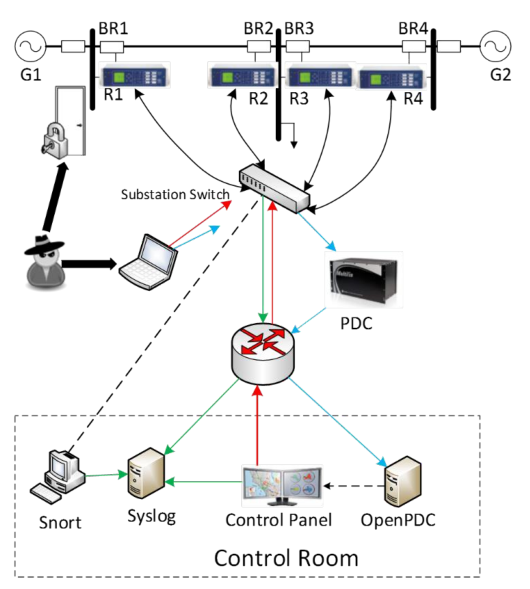
\includegraphics[width=100mm]{images/cps_rep.png}
    \caption[Power system network diagram]{Power system network diagram \cite{adhikari_power_2014}}
    \label{fig:cps_rep}
\end{figure}

The operation of this power system can be described following 6 main scenarios:
\begin{itemize}
    \item normal behaviour, 
    \item short-circuit,
    \item line maintenance,
    \item remotely opening the breakers (attack),
    \item disruption of fault protection system (attack),
    \item fault imitation (attack).
\end{itemize} 
Each of those scenarios can be divided into several sub-scenarios concerning different entities of the system or/and the failure range. Every scenario was labelled with a number between 1 and 41. In this way \textbf{37 scenarios} are obtained, divided and numbered as follows:
\begin{itemize}
    \item 1 no events scenario, its number it is 41,
    \item 8 natural fault scenarios, its number ranges are 1-6 (short-circuit) and 13-14 (line maintenance),
    \item 28 attack scenarios, its number ranges are 7-12 (fault imitation), 15-20 (remotely opening the breakers), 20-30 and 35-40 (disruption of fault protection system).
\end{itemize}
The reason for dropping the numbers between 31 and 34 in the naming process of scenarios is not known.

The datasets provided in \cite{morris_industrial_nodate} represent \textbf{78377 events}, in which one of those scenarios was reproduced in the system. They have been grouped by scenario into 3 datasets: binary (attack or normal operation), three-class (attack, normal fault and no events) and multiclass (differentiating all 37 scenarios). Each of these 3 datasets is composed of 15 .arff or .csv files comporting in average 141 events for each of 37 scenarios. The exact number of events per file for each scheme is illustrated on figure \ref{fig:scen_distro_37}. For the 3 class dataset \textbf{55663 attack}, \textbf{18309 natural fault} and \textbf{4405 normal operation} events were found. The distribution of these schemes throughout the files is shown on figure~\ref{fig:scen_distro_file}. 

\begin{figure}[H]
    \centering
    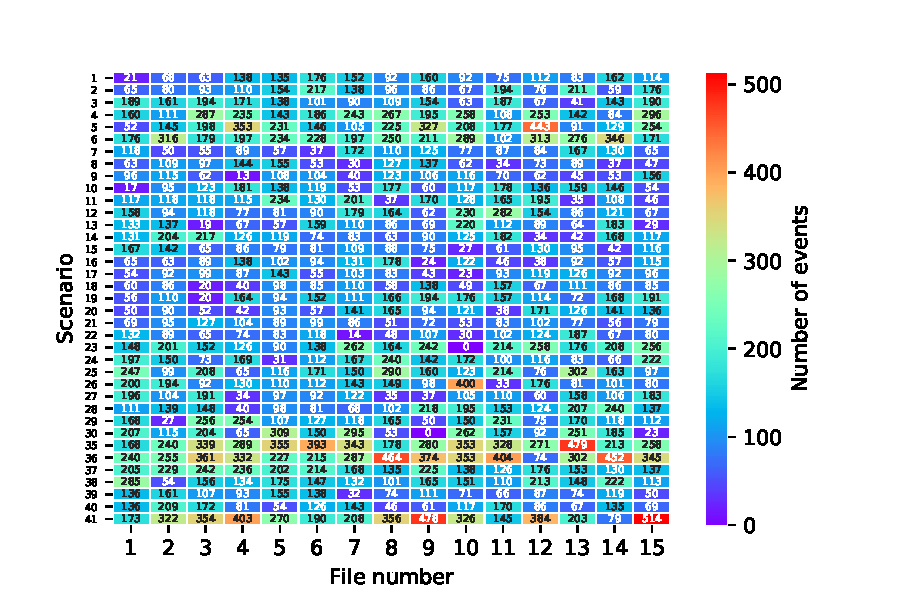
\includegraphics[]{images/distr_allscen.pdf}
    \caption{Scenarios distribution throughout all 15 files} \label{fig:scen_distro_37}
\end{figure}

\begin{figure}[H]
    \centering
    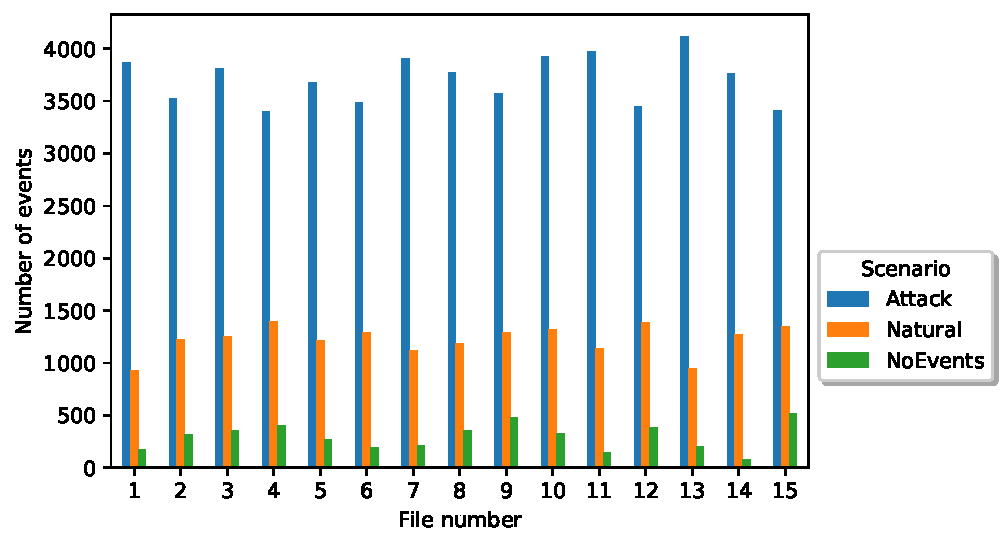
\includegraphics[]{images/distr_3classes.pdf}
    \caption{Scenarios distribution throughout the 3-class dataset files}
    \label{fig:scen_distro_file}
\end{figure}

Figure \ref{fig:scen_distro_file} shows also this distribution for the binary datasets, it is sufficient to add the number of natural (orange) and normal operation (green) events.

The scenarios are not equally distributed in the case of the 37 schemes dataset, it is especially shown by the standard deviation of 61, which is an important value compared to some scenarios counting less than 100 events. On the other hand, in the case of 3-class scenarios, the distribution is even more not equal compared to the 37 schemes dataset. The \textbf{mean standard deviation among all files is equal to 1767}, which is an enormous result given that some scenarios count only around 100 events.

Each of previously mentioned events is described by \textbf{128 features}: 116 provided by four phasor measurement units\footnote{Phasor measurement units measure the electrical waves on an electricity grid} (each one provides 29 types of measurements) and 12 other features are reserved for control panel logs, snort alerts, relay logs of 4 phasors. The mentioned 116 features, each has a label formed by \textbf{concatenation} of the \textbf{source phasor reference} (it can be R1, R2, R3, R4) and the \textbf{measurement name}, as provided in table \ref{tab:pmu_mes}. For example R4-PM5:I stands for phase B current phase magnitude measured by R4.
%give exemple - preciser plus les features 
%expliquer les features plus
%figure pour explication de phase, magnitude

\begin{table}[H]
    \centering
    \caption[Phasor measurements]{Phasor measurements \cite{adhikari_power_2014}} \label{tab:pmu_mes}
    \begin{tabular}{lr}
        \toprule
        Feature&Description \\
        \midrule
        PA1:VH – PA3:VH&Phase A-C Voltage Phase Angle \\
        PM1:V – PM3:V&Phase A-C Voltage Phase Magnitude \\
        PA4:IH – PA6:IH&Phase A-C Current Phase Angle \\
        PM4:I – PM6:I&Phase A-C Current Phase Magnitude \\
        PA7:VH – PA9:VH&Pos.–Neg.– Zero Voltage Phase Angle \\
        PM7:V – PM9:V&Pos.–Neg.–Zero Voltage Phase Magnitude \\
        PA10:VH - PA12:VH&Pos.–Neg.–Zero Current Phase Angle \\
        PM10:V - PM12:V&Pos.–Neg.–Zero Current Phase Magnitude \\
        F&Frequency for relays \\
        DF&Frequency Delta (dF/dt) for relays \\
        PA:Z&Appearance Impedance for relays \\
        PA:ZH&Appearance Impedance Angle for relays \\
        S&Status Flag for relays \\
        \bottomrule
    \end{tabular}
\end{table} 

Those datasets have been used in several works related to CPS cyber-attack classification, one of which is \cite{borges_hink_machine_2014-1}, where the author try to find the most accurate algorithm to predict the status of the power system. The following chapter shows an attempt to partially reproduce the results obtained by them.


%\appendix
\bibliography{main}
\bibliographystyle{plain}

\end{document}

